% !TeX program = lualatex
\chapter{Theoretischer Hintergrund} % Main chapter title
\label{Background} % For referencing the chapter elsewhere, use \ref{Background}
Um in den folgenden Kapiteln ein grundlegendes Verständnis der Begrifflichkeiten, Zusammenhänge und Konzepte gewährleisten zu können, ist es notwendig,
diese vorab zu definieren und einzugrenzen. Da sich diese Arbeit mit der Privatsphäre von Stakeholdern in einem Softwareentwicklungsunternehmen beschäftigt,
ist es zunächst erforderlich, die Grenzen der Privatsphäre klar zu definieren und anhand dieser, eine Messung zu schaffen. Des weiteren müssen die Stakeholder,
welche in dieser Analyse betrachtet werden, definiert, identifiziert und im weiteren Verlauf in Gruppen gegliedert werden. Im Anschluss werden DevOps definiert und anhand
gewählter Beispiele, eine Analyse dieser aufgebaut.

\section{Die Privatsphäre - eine Eingrenzung}
Der Begriff Privatsphäre ist im Wortschatz der deutschen Sprache tief verankert und findet im Alltag in vielerlei Hinsicht Gebrauch: Menschen decken Notebook- und Smartphonekameras
ab, protestieren gegen Überwachungskameras im öffentlichen Raum \cite{Stallwood:2013aa} oder möchten nicht, dass ihre persönlichen und privaten Daten auf sozialen Netzwerken ohne ihre Zustimmung
bzw. ohne ihre Kenntnis verbreitet werden \cite{Picchi:2018aa} - doch was genau bedeutet Privatsphäre? \newline
Die Privatsphäre lässt sich definieren als einen eingegrenzten, nicht-öffentlichen Raum, in welchem ein Individuum bzw. Individuen nach eigenem Belieben, ohne äußere Einflüsse oder die Beobachtung durch
Unbeteiligte, zur freien Entfaltung der eigenen Person, handeln kann \cite*{Pettinger:2020aa}. Möchte man diese Definition nun auf die Softwareentwicklung widerspiegeln, so müssen die möglichen, 
vorherrschenden Komponenten von persönlichen Daten näher betrachtet werden: In Unternehmen, welche sich mit der Softwareentwicklung befassen, müssen Daten vorhanden sein, welche Individuen individuell und 
bestimmen können (Grund liefern!) - dies kann in Form von IDs und individuell gewählten Nutzernamen vorzufinden sein, aber auf der Kehrseite auch mit Klarnamen, E-Mail Adressen sowie eindeutig identifizierbaren IDs. 

\section{Stakeholder}
Der Begriff \enquote{Stakeholder} lässt sich neben der Informatik auch in der Betriebswirtschaftslehre vorfinden - das Bindeglied der beiden Bereiche in diesem Aspekt stellen Unternehmen im Allgemeinen selbst dar.
Da diverse Institutionen, Personen und Personengruppen Erwartungen an Unternehmen haben und eigene Interessen vertreten, stellen Stakeholder jene \enquote{[...] [dar], die von den Aktivitäten eines Unternehmens 
direkt oder indirekt betroffen sind oder [...] ein Interesse an diesen [...] haben} \cite{Fleig:2016aa}. Als Beispiele können diese in Form von Kunden und Lieferanten bis zu eigenen Mitarbeitern und Eigentümern (von 
Unternehmensanteilen oder vom Unternehmen selbst) auftreten \cite{Fleig:2016aa}. \newline Neben den Stakeholdern selbst existiert der sogenannte \enquote{Stakeholder-Ansatz}: Dieser besagt die Betrachtung einer Unternehmung
als Organisation unter Zusammenschluss verschiedener Stakeholder \cite{Seyfried:2018aa}. Dabei stellt die Unternehmensleitung die Vermittlung zwischen den verschiedenen Gruppen dar \cite{Seyfried:2018aa}. \newline
Betrachtet man diesen Begriff nun aus der informatischen Sicht, so kann man aus der Definition herleiten, dass Stakeholder hier in der Regel Erwartungen und Interessen an einem einem Programm bzw. einer Applikation oder einem 
Computersystem, statt einem Unternehmen verfolgen. \newline \newline In dieser Analyse ist der Bezug fortlaufend auf diese Stakeholder gelegt.

\section{DevOps}
\enquote{Die Zufriedenheit unserer Kunden liegt uns am Herzen} - durch dieses Motto strahlen Unternehmen ihre Kundenorientierung aus und möchten in der Regel zusätzlich durch Feedback, Kulanz, einem überzeugenden Produkt
oder einem allgemein positiv zurückgebliebenem Eindruck beim Kunden überzeugen. In Softwareentwicklungsunternehmen vereint DevOps die benötigten Technologien, die Prozesse und die Menschen miteinander, um für diese Kunden 
andauernd hochwertige Produkte anbieten zu können \cite{MSAzure:2020aa}. Der Begriff setzt sich zusammen aus \enquote{Development} (dt. \textit{Entwicklung}) von Software sowie \enquote{Operations} (dt. \textit{Vorgänge}), welche damit zusammenhängen 
\cite{MSAzure:2020aa} und repräsentiert dabei die \enquote{Zusammenarbeit von Entwicklung und Betrieb} \cite{Hasselbring:2015aa} dar. Dies erfolgt durch die Einführung von DevOps-Methoden und -Tools, sodass den zuvor getrennten Bereichen, 
und zusätzlichen wie beispielsweise der Qualitätssicherung, der Sicherheit etc., die Möglichkeit zur Koordination und Zusammenarbeit geboten wird \cite{MSAzure:2020aa}. \newline \newline
Im Folgenden werden beispielhaft repräsentative DevOps-Methoden und -Tools definiert und aufgelistet.

\subsection{Continuous Integration}
In der Softwareprogrammierung ist es mit zunehmender Komplexität und Umfang des Programms üblich, mehrere einzelne Module in dieses einzubinden, weswegen sich die gängige Vorgehensweise in der Softwareentwicklung insofern gestaltet, dass das Gesamtprojekt,
welches aus diesen einzelnen Modulen besteht, durch mehrere Teams parallel vorangetrieben \cite{HJL:2018aa}. Statt auf eine täglich erfolgende Kompilierung auf einem extra angelegten \enquote{Build}-Server warten zu müssen, kommt heutzutage in modernen
Unternehmen die sogenannte \enquote{Continuous Integration} (dt. \textit{Kontinuierliche Integration}, kurz: CI) zum Einsatz \cite{HJL:2018aa}: Diese bezeichnet \enquote{eine Technik der agilen Softwareentwicklung [...], [welche die] in kleinen Schritten vorgenommenen Änderungen [...] 
regelmäßig zusammenführt} \cite{Dirk:2018aa}, also eine kontinuierliche Integration von Softwarekomponenten wie z.B. eines Guided User Interfaces (dt. \textit{grafische Benutzeroberfläche}, kurz: GUI), eines Application Programming Interfaces (dt. \textit{Programmierschnittstelle}) etc.,
in das gemeinsame Projekt bzw. den gemeinsamen Code \cite{HJL:2018aa}. Dies erfolgt in der Regel unter Einsatz von einem sogenannten \enquote{Trunk}, also der \enquote{Stamm}, welches das Hauptverzeichnis der Entwicklung des Projekts darstellt  und \enquote{Branches}, die als 
\enquote{Äste} bzw. Verzweigungen angesehen werden können und die untergeordneten Verzeichnisse der Hauptentwicklung repräsentieren \cite{Peters:2015aa}. \newline In der Arbeit im Team kann der Code dann für dasselbe Projekt also nicht erst wie zuvor nach dem Fertigstellen der anderen 
Teilbereiche mit in den Gesamtcode des Projekts aufgenommen werden, sondern nach eigenem Bedarf, sogar mehrmals am Tag \cite{Dirk:2018aa}. Dadurch kann der Code für die beteiligten Programmierer schon viel früher offengelegt werden, sodass Tests und damit verbunden, Fehlerbehebungen früher 
und effizienter durch Einsparung von Zeit und Ressourcen, durchgeführt werden können - wobei trotzdem zunächst eine Umorientierung erforderlich ist, da ein bereits gängiger Prozess neu aufgelegt und zusätzliche Prozesse sowie Server neu eingebunden werden müssen \cite{HJL:2018aa, Dirk:2018aa}. 
Dieser gesamte Prozess funktioniert durch das Einspeisen der zusammengefügten Änderungen des Codes in ein Repository, womit im Anschluss eine Versionskontrolle durch die Übernahme von einer aktuellen Version des Codes durch einen automatisierten Build-Prozess \cite{HJL:2018aa}.
\begin{marginfigure}[-1\baselineskip] % move figure up by 1 line
    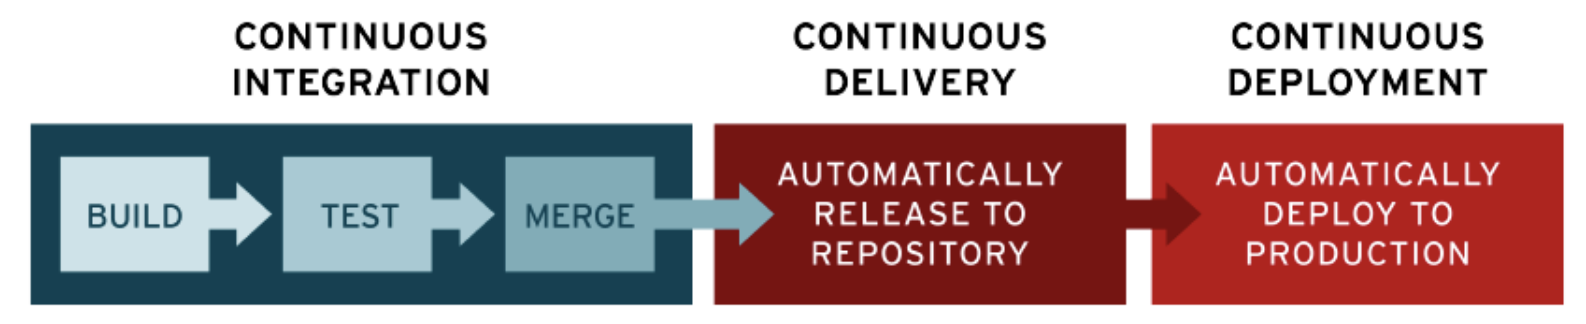
\includegraphics[width=1.3\marginparwidth]{pipeline.png}
    \caption{\label{fig:pipeline}Die CI-/CD-Pipeline.}
\end{marginfigure}

\subsection{Continuous Delivery}
Der Begriff \enquote{Continuous Delivery} (dt. \textit{Kontinuierliche Auslieferung}, kurz: CD) geht einen Schritt weiter: Eine Sammlung, welche \enquote{kurze Entwicklungszyklen und [eine] schnelle Auslieferung von Software-Updates [durch Techniken, Prozesse und Werkzeuge]} \cite{Ilanrr:2017aa}
ermöglicht, beschreibt man als Continuous Delivery. Anstatt konventionell darauf zu setzen, Software erst zu programmieren und im Anschluss einem Test und einer Evaluation zu unterziehen, bevor diese an Kunden ausgeliefert wird, kann durch Continuous Delivery eine vollfunktionsfähige Version der Software
in jedem Entwicklungsstand nach Bedarf vom Kunden bezogen werden - in der Regel ohne Fehler zu enthalten \cite{Ilanrr:2017aa}.

\subsection{Continuous Deployment}
Das Continuous Deployment (kurz: CD) stellt den Abschluss der CI-/CD-Pipeline (s. Abbildung \ref{fig:pipeline}) dar und erweitert den Continuous Delivery, welche die zur Auslieferung fertigen Builds automatisch freigibt, um die automatische Freigabe einer Applikation in der Phase der Produktion \cite{RedHat:2020aa}. Dies bedeutet in der Praxis betrachtet,
dass nach Fertigstellen der Codeänderungen und nach erfolgreichem Bestehen der definierten Tests, die Applikation automatisch (bspw. an die Kunden zum Einholen von Feedback) ausgeliefert werden kann \cite{RedHat:2020aa}.

\begin{marginfigure} % move figure up by 1 line
    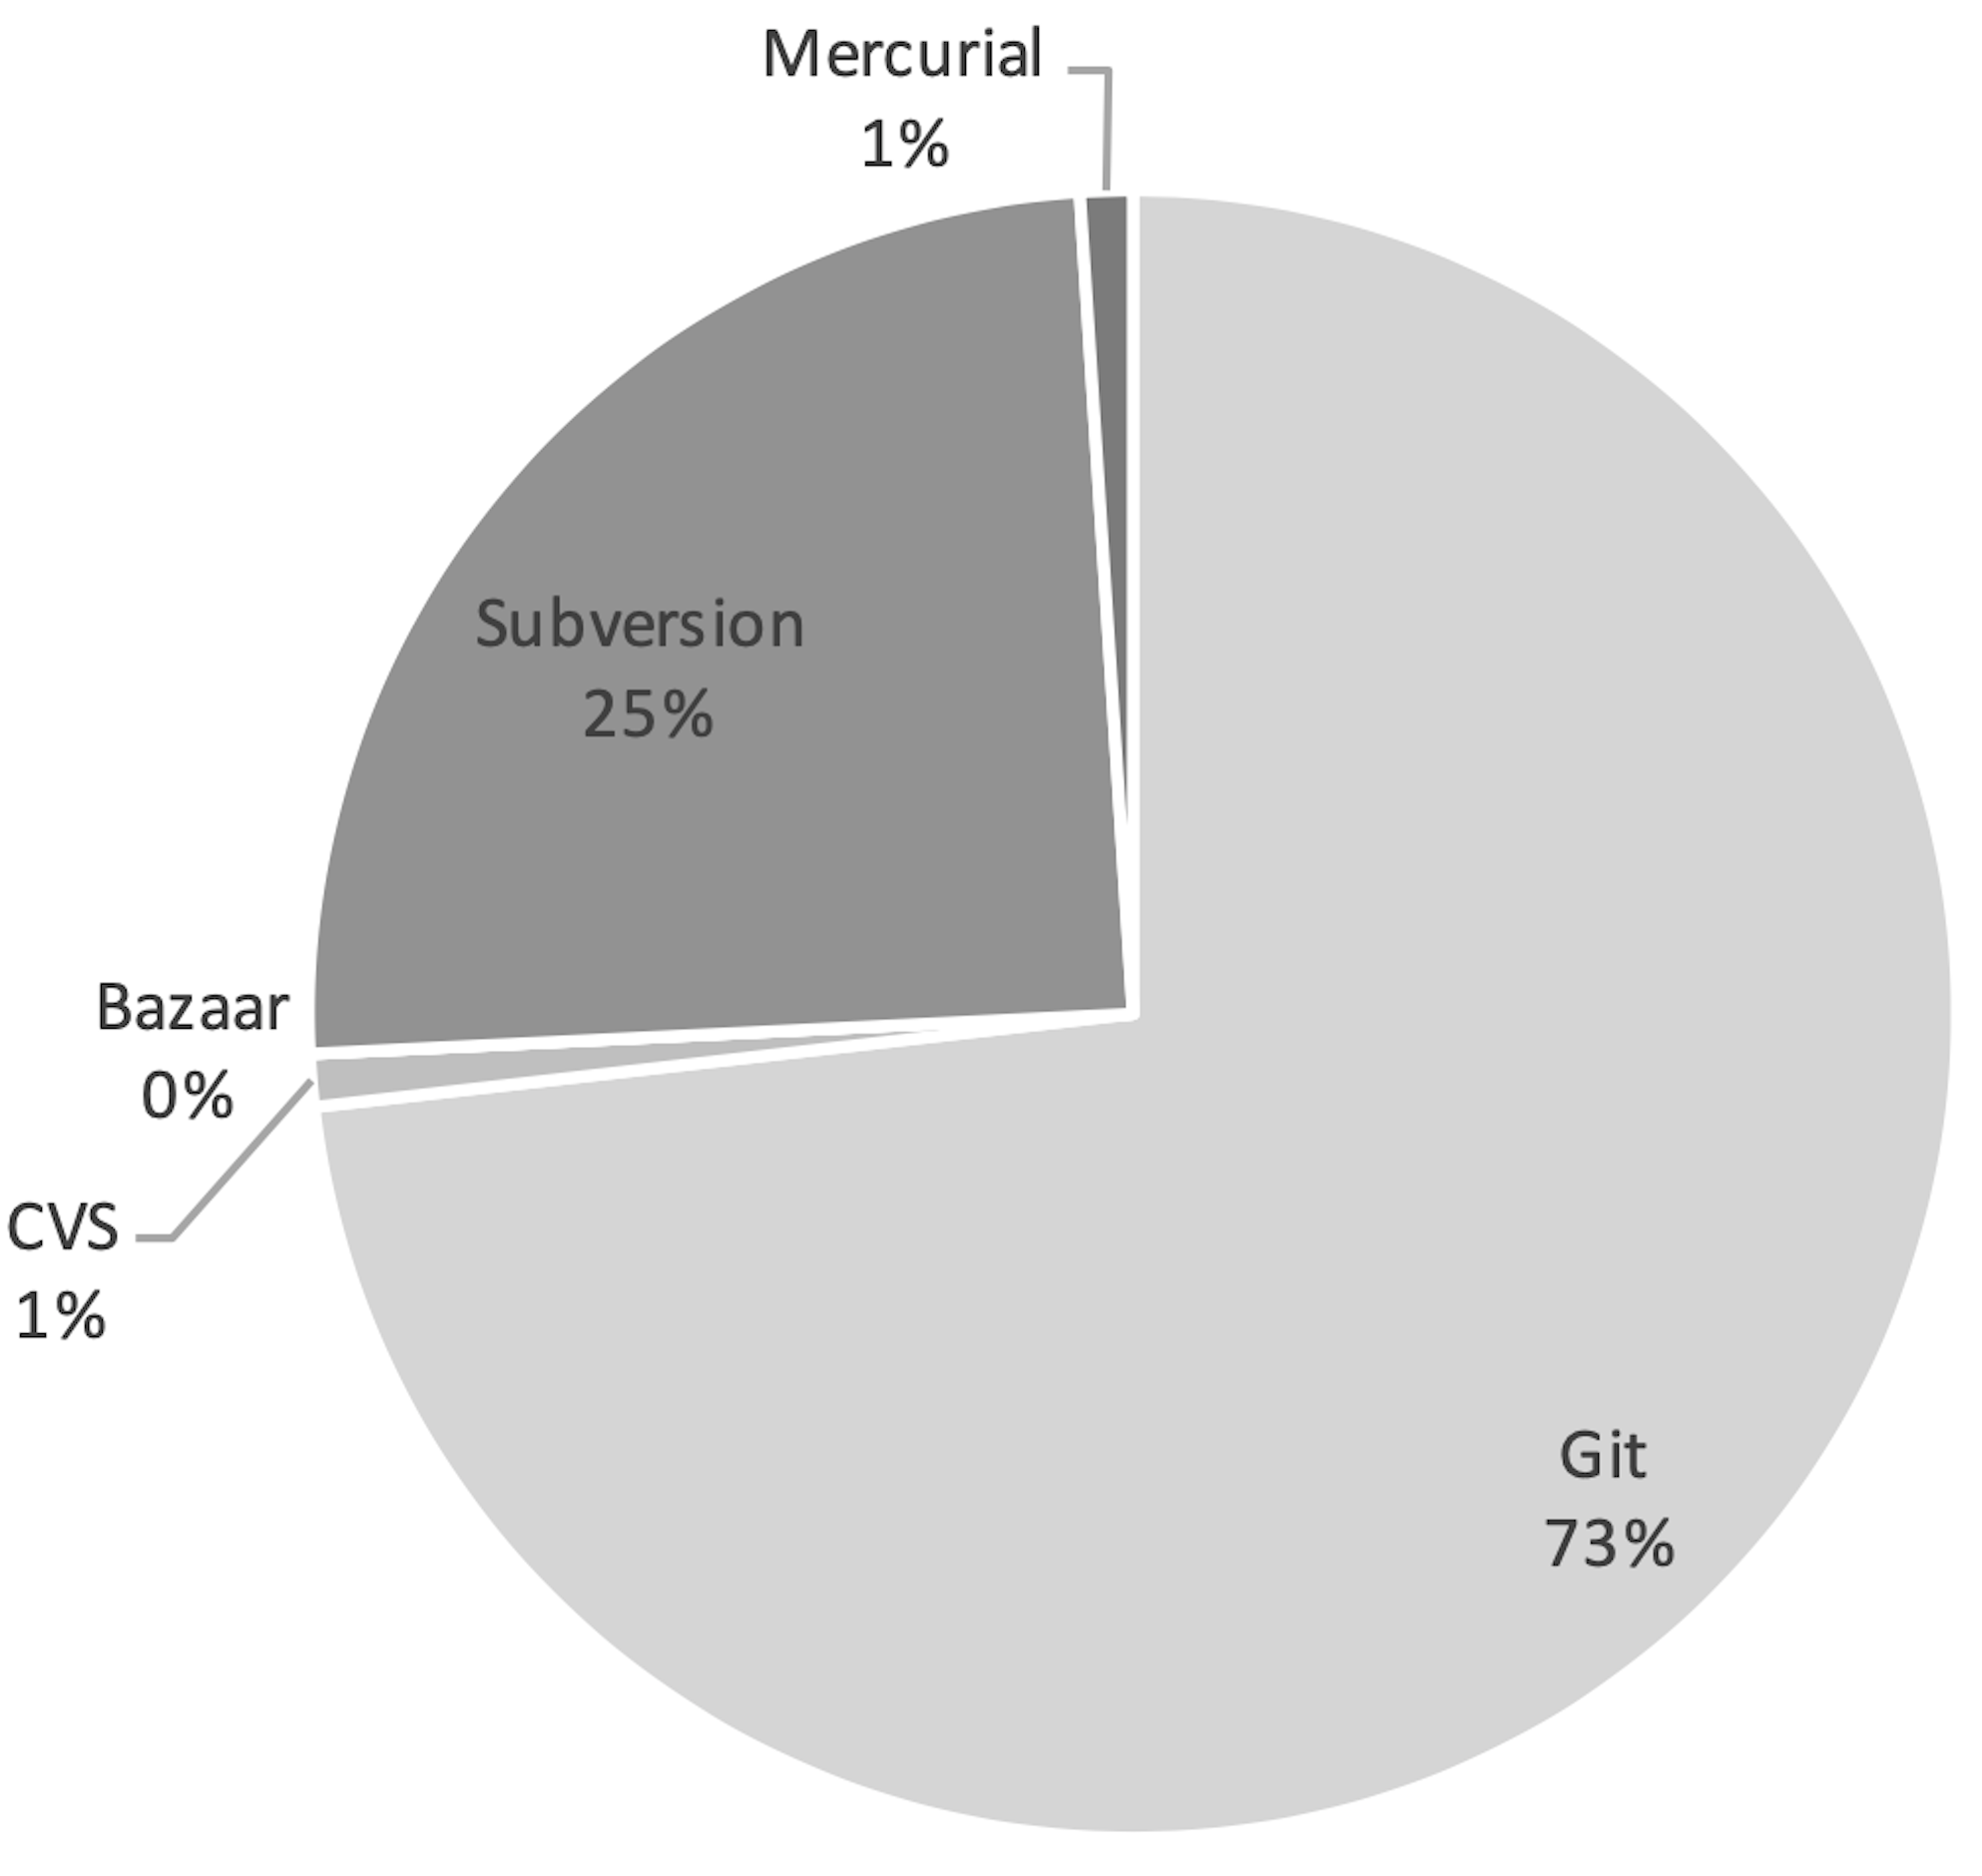
\includegraphics[width=1.1\marginparwidth]{ohloh.png}
    \caption{\label{fig:ohloh}Versionsverwaltungs-Tools im Ranking (nach Anzahl der Repositories) - Stand: 2020.}
\end{marginfigure}
\subsection{Versionsverwaltung}
Durch die Zusammenarbeit im Team an einem gemeinsamen Projekt werden Softwareentwickler häufig vor das Problem der Versionsverwaltung gestellt: Wie können mehrere Personen an einem gemeinsamen Projekt und z.T. sogar am selben Programm gleichzeitig arbeiten?
Wie können verschiedene Versionen eines Programms einheitlich und übersichtlich verwaltet werden? Und wie verfährt man möglichst effizient mit Code, welcher von unterschiedlichen Autoren geschrieben wurde und fügt diese zusammen? Zur Lösung dieser Konflikte 
ist die Versionsverwaltung heutzutage in Softwareentwicklungsunternehmen essentiell. Diese \enquote{ist ein System, welches die Änderungen an einer oder einer Reihe von Dateien über die Zeit hinweg protokolliert, sodass man später auf eine bestimmte Version 
zurückgreifen kann.} \cite{Scott-Chacon:2020aa}. Laut der Webseite Open Hub, welche zur Katalogisierung von Open-Source-Software verwendet wird und wie hier, den Anteil von Versionsverwaltungs-Tools anhand der registrierten Daten indexiert, stellen Git (71\%) 
und Subversion (24\%) die Spitze dar (s. Abbildung \ref{fig:ohloh}) \cite{Inc.:2020aa}. \newline
Git unterscheidet hierbei zwischen der lokalen, zentralen und verteilten Versionsverwaltung: Die lokale Versionsverwaltung befasst sich dabei mit der \enquote{[Verwaltung] aller Änderungen relevanter Dateien in einer Datenbank} \cite{Scott-Chacon:2020aa}, wohingegen die
zentrale mit dem Problem der Kooperation mit anderen Entwicklern an gemeinsamer Software \cite{Scott-Chacon:2020aa}. Der letzte Punkt der verteilten Verwaltung behandelt das vollständige Kopieren eines sogenannten \enquote{Repositories} (dt. \textit{Quelle bzw. Lager von Software})
von einem Server anstatt lediglich den letzten Stand zu beziehen \cite{Scott-Chacon:2020aa}.
